\newcommand{\bitmap}{\mathbb{BITMAP}}
\newcommand{\pcounting}{\textit{probabilistic counting}}

\chapter{Contagem distinta aproximada: Flajolet-Martin (1985)}
\label{lab:flajolet-martin}

\section{O Problema}

\begin{quote}
  \textbf{Contagem Distinta:} Dado um conjunto $\Mbb$, \textbf{encontrar} quantos elementos \textit{distintos}
  $\Mbb$ possui.
\end{quote}

Uma solução para a \textbf{contagem distinta} é inserir cada elemento de $\Mbb$ em uma tabela hash. 
E assim, a quantidade de itens distintos nesse conjunto será o número de elementos nessa tabela.

Note que esse algoritmo consome $\Omega(n)$ de memória, uma vez que, deve-se armazenar cada elemento 
\textbf{pelo menos uma vez} para que seja possível verificar se um item está no conjunto.

Este consumo linear de espaço pode ser um problema quando a quantidade de elementos que precisam ser armazenados é muito 
grande. E podem existir aplicações nas quais é necessário manter \textbf{várias} dessas estruturas, como no caso do 
\textit{Redis}, em que se deseja encontrar quantos usuários distintos visualizararm um publicação ~\citep{Redis}. E para 
essas situações, é interessante que o consumo de memória seja muito menor que a quantidade de elementos distintos. 
Portanto, deve-se abandonar a exatidão da contagem dos elementos distintos para que se possa diminuir o consumo de 
espaço.

\begin{quote}
  \textbf{Contagem Distinta Aproximada:} dado um conjunto $\Mbb$, \textbf{estimar} o número de elementos 
  \textit{distintos} nesse conjunto.
\end{quote}

Uma das primeiras soluções para a \textbf{contagem distinta aproximada} foi apresentada por \textit{Philippe Flajolet} e 
\textit{Nigel Martin} no artigo ~\citep{flajolet:martin:85}.
A motivação para o desenvolvimento desse algoritmo foi a otimização de pesquisas em bancos de dados relacionais.
E a identificação do número de elementos distintos em uma coluna era a principal dificuldade nesse processo.

\section{Algoritmo de Flajolet-Martin}
\label{sec:flajolet-martin:algorithm}

O \textbf{algoritmo de Flajolet-Martin} utiliza uma função de hash $h$ que associa uniformemente cada elemento do 
conjunto $\Mbb$ para um número inteiro entre $0$ e $2^L-1$, em que $L$ é a quantidade necessária de bits para 
mapear todas as entradas de $\Mbb$ (na prática, este valor é $32$ ou $64$). Assim, para cada $x_i \in \Mbb$, 
será calculado um inteiro $y_i \coloneqq h(x_i)$. Note que $y_i$ pode ser visto como uma palavra binária aleatória de 
$L$ bits em que cada bit é gerado independentemente com probabilidade $\frac{1}{2}$. E o algoritmo é baseado na 
frequência das aparições dos prefixos dessas palavras aleatórias.

Então, suponha que palavras binárias aleatórias de $L$ bits estejam sendo geradas. Espera-se que a cada \textbf{2} 
palavras, pelo menos uma comece com \textbf{1}. E que a cada \textbf{4} palavras, pelo menos uma deva ter o prefixo 
\textbf{01}. Assim, a cada $\mathbf{2^k}$ palavras, espera-se que pelo menos uma palavra comece com $\mathbf{0^{k-1}1}$. 
Por outro lado, caso o prefixo $0^{k-1}1$ apareça, o esperado é que $2^{k}$ items já devam ter sido gerados. 

Dessa forma, o algoritmo mantém a ocorrência dos prefixos de cada $\textit{hash}$ em um vetor 
$\bitmap[0 \twodots L - 1]$, de modo que $\bitmap[i] = 1$, se e somente se, o prefixo $0^i1$ apareceu entre os 
\textit{hashes} dos elementos de $\Mbb$. 

Note que é necessário mapear cada prefixo para um inteiro entre $0$ e $2^{L} - 1$. E para isso, defini-se a função $\rho$ 
que recebe um inteiro e devolve a posição do 1 menos significativo deste inteiro. Então, para um \textit{hash} $y$, 
suponha que $\rho(y) = k$. Assim, o prefixo da representação binária de $y$ é $0^k1$, e $\bitmap[k] = 1$. Um caso 
especial para essa função é quando o \textit{hash} é zero. Nesta situação, $\rho(0) = L$.

Por fim, seja $R$ o menor índice tal que $\bitmap[R] = 0$. A estimativa para o número de elementos distintos de 
$\Mbb$ será $2^R/\phi$, em que, $\phi$ é um fator de correção que será discutido em 
\refeq{sec:flajolet-martin:analysis}.

Segue o pseudocódigo:
\begin{codebox}
  \Procname{$\proc{ProbabilisticCounting}(\Mbb, h, L)$}
  \li \For i de $0$ até $L$
      \Do
  \li    $\bitmap[i] \gets 0$
      \End
  \li \For cada $x$ em $\Mbb$
      \Do
  \li   $y \gets h(x)$
  \li   $\bitmap[\rho(y)] \gets 1$
      \End
  \li $R \gets 0$
  \li \While $\bitmap[R] = 1$
      \Do
  \li   $R \gets R + 1$
      \End
  \li
  \Return $2^R/\phi$
  \End
\end{codebox}

\newpage
\section{Análise do algoritmo}
\label{sec:flajolet-martin:analysis}

Suponha que a quantidade de elementos distintos de $\Mbb$ seja $n$. O valor esperado de $R$ definido na seção 
\refeq{sec:flajolet-martin:algorithm} é aproximadamente $\log_2(\phi n)$, em que $\phi = 0.77351\dots$ e o desvio padrão 
de $R$ é em torno de $1.12$. Essa seção busca mostrar as etapas da análise do Algoritmo~\ref{prog:flajolet-martin} feita 
por Flajolet e Martin. Os detalhes da prova podem ser vistos em ~\citep{flajolet:martin:85}.

O primeiro passo é entender que $R$ é uma estimativa para $\lfloor \log_2(n) \rfloor$. Pelo padrão das aparições dos 
prefixos dos hashes dos elementos de $\Mbb$, espera-se que $\bitmap[0]$ seja acessado aproximadamente $\lfloor 
\frac{n}{2} \rfloor$ vezes, $\bitmap[1]$ aproximadamente $\lfloor \frac{n}{4} \rfloor$ vezes $\dots$ Agora, para 
$k = \lfloor \log_2(n) \rfloor$, $\bitmap[k]$ deve ser acessado em torno de $\lfloor \frac{n}{2^{k+1}} \rfloor = 0$ 
vezes. Assim, o menor índice $R$ tal que o valor de $\bitmap$ seja zero é aproximadamente $\lfloor \log_2(n) \rfloor$.

Então, defini-se a variável aleatória $R_n$ como sendo o valor da variável $R$ ao final da execução do Algoritmo 
\ref{prog:flajolet-martin} para uma entrada $\Mbb$ com $n$ elementos distintos. Dessa forma, o interesse principal 
da demonstração é encontrar fórmulas ou estimativas para:
\begin{itemize}
  \item $p_{n,k} = \mathbb{P}(R_n = k)$: probabilidade de uma saída de \ref{prog:flajolet-martin} ser igual a $k$
  \item $q_{n,k} = \mathbb{P}(R_n \geq k)$: probabilidade de uma saída de \ref{prog:flajolet-martin} 
  ser maior ou igual a $k$
  \item $\Ebb[R_n]$: valor esperado de $R_n$
  \item $\Vbb[R_n]$: variância de $R_n$
\end{itemize}

O primeiro teorema de ~\citep{flajolet:martin:85} mostra uma fórmula \textit{exata} e \textit{discreta} para $q_{n,k}$. 
A principal idea para encontrar essa fórmula é agrupar as palavras binárias por prefixos da forma $0^k1$. Assim, 
defini-se $E_k = \{ x  \ | \ \rho(x) = k \}$, ou seja, $E_k$ é o conjunto de todas as palavras aleatórias com prefixos
iguais a $0^k1$. Da mesma forma, defini-se $K_k = \{ x \ | \ \rho(x) \geq k \}$. Em seguida, as diferentes entradas 
$\Mbb$ com $n$ elementos distintos são representadas por um polinômio:
\[ P_k^{(n)} = (E_0 + E_1 + \twodots + E_{k-1} + K_k)^n .\]

O próximo passo é tentar expandir esse polinômio usando \textit{inclusão e exclusão}, e associar uma medida 
probabilidade para $E_0, E_1, \twodots, E_{k-1}, K_k$. E a prova deste teorema termina encontrando uma relação entre 
$q_{n,k}$ e esta expansão de polinômio.

Em seguida, o Teorema 2 apresenta aproximações de $q_{n,k}$ para diferentes intervalos de $k$. E a consequência deste 
teorema é a existência de uma distribuição limitante para a distribuição de probabilidade de $R_n$ conforme $n$ cresce. 
Dessa forma, obtém-se uma fórmula \textit{aproximada} e \textit{contínua} para $q_{n,k}$:
\[ q_{n,k} \approx \psi(\frac{n}{2^k}) \]

em que, $\psi(x) = \prod_{j \geq 0} (1 - e^{-x2^j})$.

Note que por definição, $p_{n,k} = q_{n,k} - q_{n,k+1}$. Assim, pode-se aproximar $p_{n,k}$:
\[ p_{n,k} \approx \psi(\frac{n}{2^k}) - \psi(\frac{n}{2^{k+1}}) \ . \]

O interesse passa a ser, portanto, estimar $\Ebb[R_n]$ a partir dessa fórmula aproximada de $p_{n,k}$, de maneira 
que 
\[ \Ebb[R_n] = \sum_{k \geq 1} k p_{n,k} \approx \sum_{k \geq 1} k \Big[ \psi \Big( \frac{n}{2^k} \Big) - \psi 
  \Big( \frac{n}{2^{k+1}} \Big) \Big] \ . \]

Desse modo, defini-se a função real $F(x)$ como sendo
\[ F(x) =  \sum_{k \geq 1} k \Big[ \psi \Big( \frac{n}{2^k} \Big) - \psi \Big( \frac{n}{2^{k+1}} \Big) \Big] \ . \]

E o Lema 1 do artigo, afirma que 
\[ \Ebb[R_n] = F(x) + O \Big( \frac{1}{n^{0.49}} \Big) \ , \]
ou seja, que o valor esperado de $R_n$ se aproxima de $F(x)$ conforme $n$ cresce.

Em seguida, o Lema 2 apresenta o resultado da \hyperref[ap:mellin]{transformada de Mellin} de $F(X)$. A principal razão 
para se calcular essa transformação é que se pode expressar a fórmula inversa da transformada de Mellin como uma 
expansão assintótica cujos termos são resíduos da transformada. Assim, o Teorema $3A$ utiliza os Lemas 1 e 2, e o 
Teorema dos Resíduos para afirmar que 
\[ \Ebb[R_n] = \lg (\phi n) + P(\lg n) + o(1) \ , \]
em que, $P(x)$ é a expansão assintótica de $F(x)$ e $\phi = 0.77351\dots$, concluindo a prova que 
$\Ebb[R_n] \approx \lg (\phi n)$.

A prova para a estimativa de $\Vbb[R_n]$ segue os mesmos passos da prova anterior. Pela definição de 
\hyperref[ap:variance]{variância}, precisa-se estimar $\Ebb[R_n ^ 2]$. Assim, 
\[ \mathbb{E[R_n ^2]} = \sum_{k=1} k^2 p_{n,k} \approx G(x) \ , \]
em que
\[ G(x) = \sum_{k=1} k^2 p_{n,k} \ . \]

Dessa forma, encontra-se a transformada de Mellin de $G(x)$ e se analisa a inversa desta transformação para estimar 
$\Ebb[R_n^2]$.

\section{Melhorando precisão do algoritmo}

Na seção anterior, foi visto que $\Ebb[R_n] \approx \lg(\phi n)$, em que $\phi \approx 0.77351$. Assim, se o valor 
do contador $R$ no final do Algoritmo \ref{prog:flajolet-martin} para uma entrada com $n$ elementos distintos for 
aproximadamente igual a $\lg(\phi n)$, então a saída desse algoritmo é aproximadamente $n$. A tabela \ref{tab:flajolet} 
mostra que, em alguns casos, a saída do programa é praticamente igual a $n$ quando $R_n \approx \lg(\phi n)$.

\begin{center}
  \def\arraystretch{2}%
  \begin{table}
    \begin{tabular}{ |p{1.5cm}||p{2.5cm}|  }
      \hline
      \multicolumn{1}{|p{1.5cm}|}{\centering $n$ } 
      & \multicolumn{1}{|p{2.5cm}|}{\centering $(1 \slash \phi) 2^{\lg(\phi n)}$ }  \\
      \hline
      \multicolumn{1}{|p{1.5cm}|}{\centering 50 } 
      & \multicolumn{1}{|p{2.5cm}|}{\centering 49.99 }  \\
      \hline
      \multicolumn{1}{|p{1.5cm}|}{\centering 500 } 
      & \multicolumn{1}{|p{2.5cm}|}{\centering 500.0 }  \\
      \hline
      \multicolumn{1}{|p{1.5cm}|}{\centering 5000 } 
      & \multicolumn{1}{|p{2.5cm}|}{\centering 4999.99 }  \\
      \hline
      \multicolumn{1}{|p{1.5cm}|}{\centering 50000 } 
      & \multicolumn{1}{|p{2.5cm}|}{\centering 50000.0 }  \\
      \hline
     \end{tabular}
     \caption{\label{tab:flajolet} Comparação entre $n$ e saída do Algoritmo \ref{prog:flajolet-martin} para 
     $R_n = \lg(\phi n)$.}
  \end{table}
\end{center}

Contudo, $\Vbb[R_n] \approx\nolinebreak 1.12$ e consequentemente, o desvio padrão de $R_n$ é aproximadamente~$1$. 
Isto quer dizer que o valor de $R_n$ pode ser uma unidade maior ou menor que $\lg(\phi n)$, o que implica que a 
estimativa de $n$ possa ser duas vezes maior ou menor que $n$. Logo, o Algoritmo de Flajolet e Martin apresenta uma 
grande variabilidade.

Assim como foi visto na Seção \ref{sec:morris:plus}, pode-se diminuir a variância da estimativa fazendo $k$ iterações 
do Algoritmo \ref{prog:flajolet-martin}. Dessa forma, seria necessário manter $k$ vetores $\bitmap$, $k$ valores de $R$ e 
$k$ funções de hash $h$. Ao final de todas as $k$ iterações, seria calculado a média $\bar{R}$ dos valores de $R$, e a 
estimativa do número de elementos distintos seria $(1 \slash \phi) 2^{\bar{R}}$.

O pseudocódigo a seguir codifica essa idea:
\begin{codebox}
  \Procname{$\proc{ProbabilisticCounting+}(\Mbb, m, \mathbb{H}, L)$}
  \li \For $i$ de $0$ até $m$
      \Do
  \li    \For $j$ de $0$ até $L$
          \Do
  \li       $\mathbb{BITMAP}_{i}[j] \gets 0$
          \End
      \End
  \li \For $i$ de $0$ até $m$
      \Do
  \li    \For cada $x$ em $\Mbb$
          \Do
  \li       $y \gets \mathbb{H}_{i}(x)$
  \li       $\bitmap_i[\rho(y)] = 1$
          \End
      \End
  \li \For $i$ de $0$ até $m$
      \Do
  \li    $\mathbb{R}[i] = 0$
      \End
  \li $\bar{R} = 0$
  \li \For de $i$ até $m$
      \Do
  \li $\bar{R} = \bar{R} + \mathbb{R}[i]$
      \End
  \li $\bar{R} = \bar{R} / m$
  \li
  \Return $2^{\bar{R}}/\phi$
  \End
\end{codebox}

Seja $\bar{R_n}$ o valor da variável $\bar{R}$ ao final da execução do Algoritmo \ref{prog:flajolet-martin+} para uma
entrada com $n$ elementos distintos. De forma análoga aos resultados vistos na Seção \ref{sec:morris:plus}, pode-se
concluir que:
\[ \Ebb[\bar{R_n}] \approx \lg(\phi n)  \; \; \text{e}  \; \; \Vbb[\bar{R_n}] \approx \frac{1.12}{k} \ . \]


No entanto, o fato de se precisar de uma função de hash distinta para cada iteração torna a solução acima inviável, 
uma vez que, encontrar funções de hash que mapeiem na prática os elementos de um conjunto $\Mbb$ de maneira
uniforme não é uma tarefa simples. Para contornar esse problema, os autores propuseram o uso da 
\textit{média estocástica}.

Essa ideia consiste em dividr os elementos da entrada em $k$ lotes e usar parte da informação do hash para definir em 
qual lote um elemento deve ir. 
As linhas de $7$ até $11$ do pseudocódigo a seguir mostram como esta divisão é feita:
\begin{programruledcaption}{
  Algoritmo de Flajolet-Martin++
  \\ \textbf{Entrada:} conjunto $\Mbb$, funções de hash $h$, tamanho $L$ do vetor $\bitmap$, 
  quantidade $k$ de lotes
  \\ \textbf{Saída:} quantidade de elementos distintos de $\Mbb$
  \label{prog:flajolet-martin++}
  }
    \begin{lstlisting}[
      language={[brazilian]pseudocode},
      style=pseudocode,
      style=wider,
      functions={},
      specialidentifiers={},
    ]
        funcao FlajoletMartin($\Mbb$, k, h, L)
          para i de 0 até k \kw{faça}:
            para j de 0 até L \kw{faça}:
              $\bitmap_i[j]$ := 0
            fim
          fim
          para x $\in$ $\Mbb$ \kw{faça}:
            lote := $h(x) \mod k$
            y := $\lfloor h(x) / k \rfloor$
            $\bitmap^{<lote>}[\rho(y)]$ := 1
          fim
          para i de 0 até k \kw{faça}:
            $R_i$ := 0
          fim
          para i de 0 até k \kw{faça}:
            enquanto $\bitmap_i[R_i]$ = 1 \kw{faça}:
              $R_i$ := $R_i$ + 1
            fim
          fim
          $\bar{R}$ := 0
          para i de 0 até k \kw{faça}:
            $\bar{R}$ := $\bar{R} + R_i$ 
          fim
          $\bar{R}$ := $\bar{R} \slash k$
          devolva $k2^{\bar{R}}/\phi$
        fim
    \end{lstlisting}
  \end{programruledcaption}

Se a função de hash $h$ distribuir os $n$ elementos distintos do conjunto $\Mbb$ uniformemente entre os 
$k$ lotes, então espera-se que cada lote tenha aproximadament $\frac{n}{k}$ elementos. Dessa forma, 
$(1 / \phi)2^{\bar{R_n}}$ seria uma aproximação para $\frac{n}{k}$. É devido a este fato que a saída do Algoritmo~
\ref{prog:flajolet-martin++} é $\mathbf{k} (1 / \phi)2^{\bar{R_n}}$, pois este valor é uma estimativa para 
$\mathbf{k} \frac{n}{k} = n$.

Por fim, o erro relativo esperado do algoritmo \proc{ProbabilisticCounting++} é em torno de $0.78 / \sqrt{m}$. Isto quer 
dizer que para $m = 64$, o desvio esperado é em torno de $10\%$. Dessa forma, a escolha de $m$ depende das exigências do 
problema. Se precisarmos de uma precisão maior, escolheremos um valor de $m$  maior, mas teremos um algoritmo mais 
custoso em termos de tempo e espaço. Por outro lado, se a exigência é, por exemplo, decidir qual de dois conjuntos tem a 
menor quantidade de elementos distintos, podemos escolher um valor menor de $m$ para fazer essa comparação, mas teríamos 
um risco maior de escolher o conjunto errado.

\section{Limitações do algoritmo $\pcounting$}

Uma das principais razões para escolhermos algoritmos \textit{probabilísticos} ao invés de algoritmos \textit{exatos} é 
o \textbf{consumo de memória reduzido}. Por exemplo, para resolver o problema da contagem distinta de forma 
\textit{exata}, podemos manter uma tabela de hash e conforme os elementos forem processados, adicionar a esta tabela 
somente aqueles elementos que não apareceram ainda. Assim,  quantidade de elementos distintos processados será o tamanho 
da tabela. Suponha que cada hash seja um inteiro de 4 bytes (32 bits) e que existam um milhão de itens distintos 
percorridos. Para armazenar essa tabela, gastaríamos pelos menos 4 MB. Por outro lado, se usarmos o algoritmo 
$\pcounting$ para resolver esse problema, o consumo de memória seria proporcional ao valor $m$ e não dependeria da 
quantidade de itens distintos. Logo, se o vetor $\bitmap$ for um vetor de inteiros de 4 bytes de tamanho $m$, e 
$m$ for igual a 1024, então a memória consumida por esse algoritmo seria em torno de 4 KB, que é um consumo de espaço
\textbf{1000 vezes menor} que a solução exata.

O erro relativo esperado do $\pcounting$ para $m = 1024$ é em torno de $2{,}5\%$. Assim, para um conjunto de milhões de 
itens distintos, o erro seria em torno das dezenas ou centenas de milhares. Com esse tipo de desvio, teríamos como 
mensurar a ordem de grandeza do número de itens distintos de um conjunto com bastante confiança. Contudo, para utilizar
o $\pcounting$, o viés desse algoritmo deve ser entendido.

O \textbf{viés} de um estimador é a diferença entre seu valor esperado e o valor real do parâmetro estimado. 
Nesse sentido, a estimativa da quantidade de elementos em um conjunto devolvida pelo algoritmo de \proc{Morris} é 
\textit{não-viesada}, uma vez que, o Lema \ref{morris:expected_value} afirma que o valor esperado deste estimador é 
igual ao tamanho do conjunto estimado.

Na prova descrita em ~\citep{flajolet:martin:85}, o estimador de $\lg(n)$ é $R_n$, que representa o valor da variável 
$R$ ao final da execução de \proc{ProbabilisticCounting}, tendo como entrada um conjunto com $n$ elementos distintos. 
Vimos que o valor esperado de $R_n$ é aproximadamente $\lg(\phi n)$, que é diferente de $\lg(n)$. Portanto, $R_n$ é um 
estimador \textit{viesado} de $\lg(n)$. E analogamente, o estimador devolvido por \proc{ProbabilisticCounting++} também 
é \textit{viesado}.  

Então, além do erro padrão, existe também o viés do algoritmo $\pcounting$, cujo valor é $1 + 0{,}31/m$. Contudo, para 
valores de $m$ maiores que $32$, o viés se torna desprezíval se comparado ao erro padrão. Dessa forma, uma pessoa pode 
ser induzida a concluir que a escolha de $m$ é o único cuidado que ela deve tomar ao utilizar esse algoritmo. No 
entanto, ainda existe o problema de estimar \textit{baixas cardinalidades} com essa estrutura.

Suponha, portanto, que $m = 64$ e que o hash do único elemento de um conjunto $\Mbb$ comece com $1$. Logo, se passarmos 
$\Mbb$ para \proc{ProbabilisticCounting++}, existiria um vetor $\bitmap$ cuja primeira posição teria o valor $1$, e o 
restante dos vetores $\bitmap$ teriam todos valores zero. Assim, $\bar{R}$ seria igual a $1/64$, e o estimador de $n$ 
teria o valor de $64 \ 2^{\frac{1}{64}}/\phi \approx 83.64$. Esta estimativa está muito distante do valor real, que é 
$n = 1$.

Em vista disso, um tratamento especial deve ser dado para situações em que a cardinalidade do número de elementos 
distintos de um conjunto for baixa. Poderíamos, por exemplo, manter os elementos percorridos em uma tabela de hash, e 
quando essa tabela atingisse um certo tamanho, passaríamos a usar a estratégia original do $\pcounting$, que é preencher
os vetores $\bitmap$.  

\section{Simulação do algoritmo $\pcounting$}

Nesta seção, vamos ver os resultados de simulações do $\pcounting$, em que, um milhão de inteiros gerados 
aleatoriamente foram inseridos em uma implementação dessa estrutura. 

Esta implementação é baseada no pseudocódigo do \proc{ProbabilisticCounting++}. Contudo, enquanto que 
nesse pseudocódigo, o $\pcounting$ é descrito como uma função que recebe um conjunto e retorna o número de elementos 
distintos deste conjunto, o código utilizado nas simulações utiliza uma abordagem voltada à orientação a objetos. Nesse 
sentido, definimos uma classe \textit{ProbabilisticCounting}, cujo construtor recebe os parâmetros $m$ e $L$. E nesta 
classe, existem os métodos \textit{add} e \textit{count}. O primeiro adiciona um elemento à estrutura, e o segundo 
devolve a estimativa do valor de elementos distintos. Dessa forma, as simulações se baseiam em uma versão 
\textit{online} do $\pcounting$ para que possamos observar como a estimativa evolui conforme novos itens são inseridos 
nessa estrutura.

O valor de $L$ utilizado nas simulações foi de $32$, uma vez que, nas linguagens de programação, um inteiro é geralmente 
armazenado em $4$ bytes de memória. Já os valores de $m$ escolhidos foram 64 e 1024. Com estes valores, podemos ver 
a evolução da precisão da estimativa conforme $m$ aumenta. Outro detalhe de implementação é que não estamos utilizando a 
função de hash~$h$ durante a inserção dos elementos na estrutura, uma vez que, os elementos inseridos já são inteiros e 
assim, não há a necessidade de mapeá-los para inteiros entre $0$ e $2^{32} - 1$.

O gráfico a seguir exibe a evolução da estimativa conforme itens vão sendo inseridos na estrutura com $m = 64$. Observe 
que até setecentos mil elementos, a estimativa se manteve dentro da faixa do erro relativo teórico esperado, que é em 
torno de $5\%$. Mas a partir desse ponto, o erro passou a ser maior que o esperado, ultrapassando o valor de $10\%$. 
Uma das possíveis razões para essa situação é que um inteiro $x$ com um grande valor de $\rho(x)$ pode ter aparecido 
antes do esperado, o que faz com que a estimativa aumente drasticamente.

\begin{figure}
  \centering
  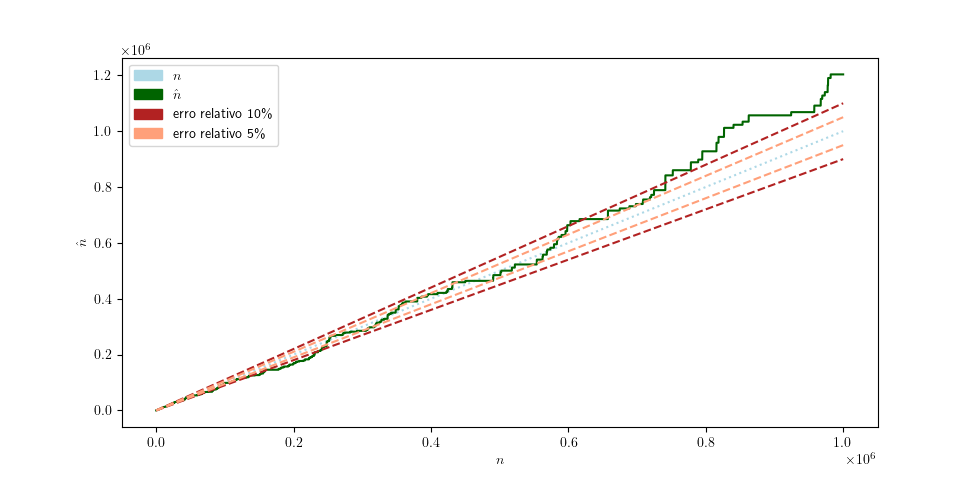
\includegraphics[scale=0.50]{figuras/pcounting-estimate-64.png}
	\caption{Evolução da estimativa do $\pcounting$ com $m = 64$}
  \label{fig:pcounting:64}
\end{figure}

\newpage
Os próximos gráficos mostram, respectivamente, a porção inicial do gráfico acima e a evolução do erro relativo nessa 
faixa, que corresponde às 256 primeiras estimativas. É possível, dessa forma, notar que o $\pcounting$ é pouco preciso 
para estimar cardinalidades baixas, podendo o erro relativo ser maior que $1000\%$ nessas situações.

\begin{figure}
  \centering
  \subfloat[\centering Evolução da estimativa $(m=64)$]{{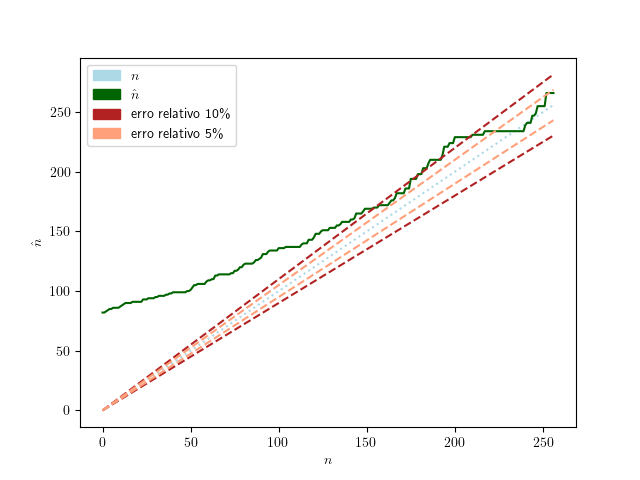
\includegraphics[width=7cm]{figuras/pcounting-estimate-64-first.png} }}
  \qquad
  \subfloat[\centering Evolução do erro relativo $(m=64)$]{{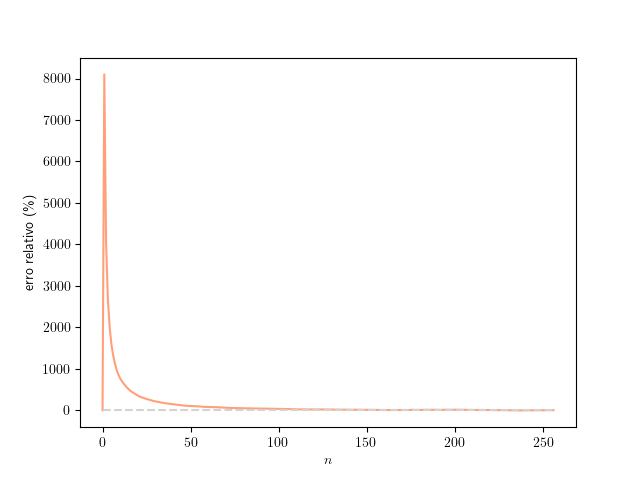
\includegraphics[width=7cm]{figuras/pcounting-error-64-first.png} }}
  \caption{Resumo das primeiras 256 estimativas}
  \label{fig:pcounting:64:first}
\end{figure}

Então, podemos aumentar o valor do parâmetro $m$ para tentar corrigir esses problemas de precisão. O gráfico seguinte 
mostra uma simulação em que os mesmos elementos da primeira simulação foram inseridos em uma estrutura com $m = 1024$.
Comparando o gráfico abaixo com a Figura \refeq{fig:pcounting:64}, nota-se que a precisão das estimativas de 
cardinalidades maiores que setecentos mil melhoraram quando o valor de $m$ foi aumentado, e o erro para essas 
cardinalidades altas ficou na faixa de $10\%$. Contudo, o erro ainda ficou acima do erro relativo esperado para 
$m = 1024$, que é aproximadamente~$2{,}5\%$.

\begin{figure}
  \centering
  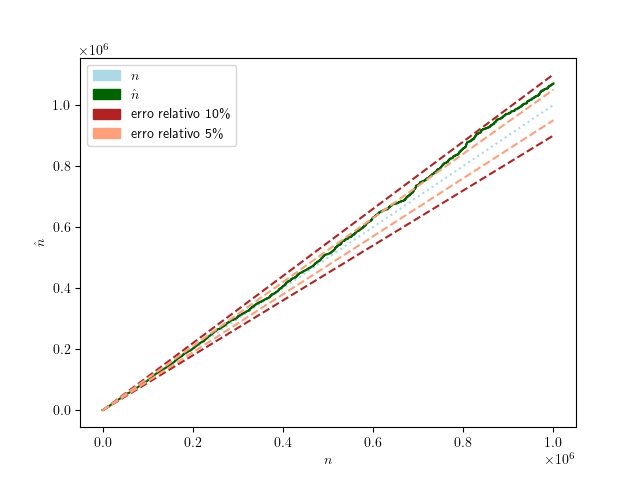
\includegraphics[scale=0.50]{figuras/pcounting-estimate-1024.png}
	\caption{Evolução da estimativa do $\pcounting$ com $m = 1024$}
\end{figure}

\newpage

Os dois últimos gráficos resumem o comportamento do $\pcounting$ com $m = 1024$ para cardinalidades baixas. Novamente, a
faixa escolhida para as construções desses gráficos foi as primeiras 256 estimativas. E o erro para estimar essas 
cardinalidades aumentou se comparado com o erro da estrutura com $m = 64$.

\begin{figure}
  \centering
  \subfloat[\centering Evolução da estimativa $(m=1024)$]{{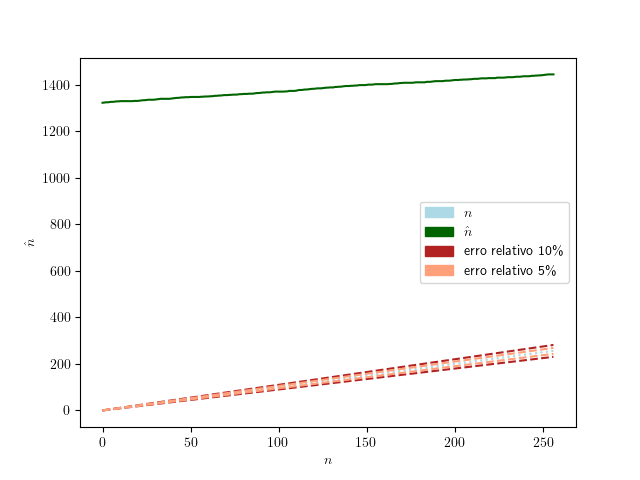
\includegraphics[width=7cm]{figuras/pcounting-estimate-1024-first.png} }}
  \qquad
  \subfloat[\centering Evolução do erro relativo $(m=1024)$]{{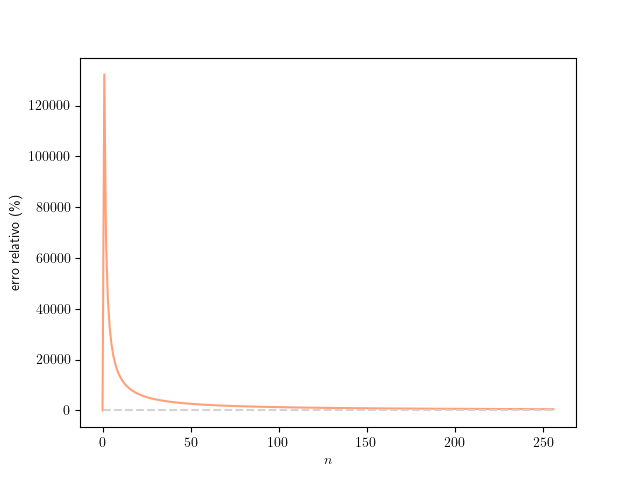
\includegraphics[width=7cm]{figuras/pcounting-error-1024-first.png} }}
\end{figure}

A precisão do $\pcounting$, portanto, pode ser melhorada se aumentarmos o valor de $m$, mas essa ideia não se aplica 
para cardinalidades baixas. O artigo ~\citep{flajolet:martin:85} nomeia esse problema como 
\textit{não-lineariade inicial}, e os autores afirmam que a estimativa se aproxima do valor esperado do estimador assim 
que a cardinalidade estimada atinge pelo menos os valores $10m{-}20m$. Assim, para $m = 64$, é esperado que essa 
imprecisão inicial desapareça por volta de seiscentos itens, e pela Figura \ref{fig:pcounting:64:first}, vemos que esse 
problema desapare por volta de cento e cinquenta itens.

Vale lembrar, no entanto, que a proposta inicial para a adoção de estruturas de dados probabilísticas é o alto consumo 
de memória conforme o volume dos dados cresce. Nesse sentido, esse problema da \textit{não-linearidade inicial} pode ser 
desconsiderado dependendo da situação. 

Por fim, o $\pcounting$ foi um dos primeiros algoritmos que surgiram para resolver o problema da 
\textbf{Contagem Distinta Aproximada}, e até nos dias atuais, é uma das estruturas com o menor erro relativo esperado, 
que é igual a $0.78 / \sqrt{m}$. Embora o $\pcounting$ não seja tão utilizado atualmente, o seu desenvolvimento serviu 
de base para que outras estruturas com menor consumo de memória surgissem, e a análise delas é muito semelhante à 
análise presente em ~\citep{flajolet:martin:85}. 